\documentclass[11pt]{article}
\usepackage[letterpaper,margin=0.7in]{geometry}
\usepackage[T1]{fontenc}
\usepackage[sc]{mathpazo}\linespread{1.0}
\usepackage{xcolor,amssymb,amsmath,graphicx,microtype,enumitem,booktabs}
\usepackage[font=small,labelfont=bf,skip=4pt]{caption}
\usepackage[colorlinks,urlcolor=blue!50!black,linkcolor=black]{hyperref}
\usepackage{titlesec}
\titleformat{\section}{\normalsize\bfseries}{}{0pt}{}
\titlespacing*{\section}{0pt}{10pt}{3pt}
\setlength{\parskip}{4pt}\setlength{\parindent}{0pt}
\pagestyle{plain}\raggedbottom
\begin{document}
\begin{center}
{\Large\bfseries The Kelvin--Helmholtz Instability\\[2pt] with a 2D Finite-Volume Euler Solver}\\[6pt]
{\small Aryana Haghjoo \;\textperiodcentered\; Astrophysical Fluid Dynamics, Assignment 2 \;\textperiodcentered\; October 2026}
\end{center}

\section{1. Goal and setup}
I built a 2D compressible hydrodynamics code following P.~Mocz's finite-volume tutorial and used it to simulate the Kelvin--Helmholtz (KH) instability, the classic shear-flow instability and a standard test of hydro codes.

The code solves the ideal Euler equations (conservation of mass, momentum and energy) for an ideal gas with $\gamma=5/3$, in a periodic unit box:
\begin{itemize}[nosep,leftmargin=*]
\item a dense band ($\rho=2$) moving right at $v_x=+0.5$ occupies $0.25<y<0.75$;
\item lighter gas ($\rho=1$) moving left at $v_x=-0.5$ surrounds it;
\item the pressure is uniform, $P=2.5$, so the shear is subsonic (Mach number $0.25$--$0.35$);
\item the two interfaces are seeded with $v_y=w_0\sin(4\pi x)$, Gaussian-localized around $y=0.25$ and $0.75$. That puts two wavelengths across the box.
\end{itemize}

\section{2. Method}
The scheme is a second-order \textbf{MUSCL--Hancock} finite-volume method. Each time step:
\begin{enumerate}[nosep,leftmargin=*]
\item converts the conserved variables to primitive ones $(\rho, v_x, v_y, P)$;
\item sets the time step by the CFL condition, $\Delta t = 0.4\,\min\!\left[\Delta x/(c_s+|\mathbf v|)\right]$;
\item computes cell gradients by central differences, optionally slope-limited;
\item advances the primitives by $\Delta t/2$ using the primitive-form Euler equations (the ``predictor'');
\item linearly extrapolates them to the left and right states at each cell face;
\item computes face fluxes with the Rusanov (local Lax--Friedrichs) Riemann solver, then updates each cell by flux in minus flux out.
\end{enumerate}
Steps 4--5 make the method second order in space and time. Because step 6 is in flux form, mass, momentum and energy are \textbf{conserved to round-off}. Over every run the relative changes in total mass and energy were $\lesssim10^{-16}$.

\section{3. Results: evolution}
The seeded ripples grow, steepen and roll up into the characteristic KH ``cat's-eye'' billows by $t\approx1$. By $t=2$ they have wound into vortices that stir the two streams together (Fig.~\ref{fig:rho}, top row).

\begin{figure}[!t]
\centering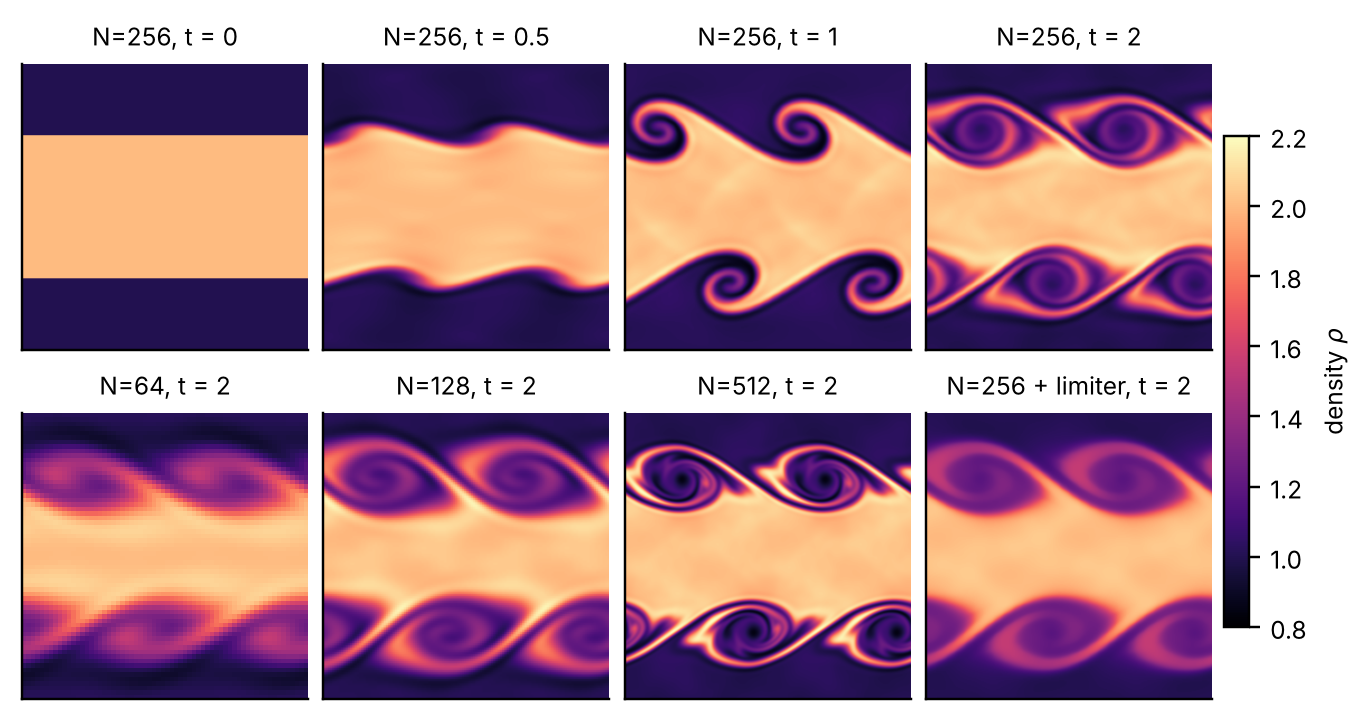
\includegraphics[width=0.88\textwidth]{fig_density.png}
\caption{Density. \textit{Top:} evolution of the fiducial run ($N=256^2$, $w_0=0.1$). \textit{Bottom:} the state at $t=2$ at different resolutions, and with the slope limiter switched on.}
\label{fig:rho}
\end{figure}

\textbf{Resolution and slope limiter} (Fig.~\ref{fig:rho}, bottom row). The large-scale billows look the same at all resolutions, but the fine structure does not converge: the interfaces get sharper and secondary instabilities appear as $N$ grows. Switching on the slope limiter suppresses spurious oscillations at the interfaces. It is also visibly more diffusive, blurring the vortex cores about as much as halving the resolution.

\section{4. Results: linear growth rate}
To test the code quantitatively, I reran with a small seed ($w_0=10^{-3}$) and measured the exponential growth of the $k=4\pi$ Fourier mode of $v_y$ (Fig.~\ref{fig:growth}). Linear theory for a sharp, incompressible vortex sheet predicts
\[
\sigma = k\,\Delta U\,\frac{\sqrt{\rho_1\rho_2}}{\rho_1+\rho_2} = 4\pi\cdot1\cdot\frac{\sqrt2}{3}\approx 5.92 .
\]

\begin{figure}[!h]
\centering
\begin{minipage}{0.46\textwidth}
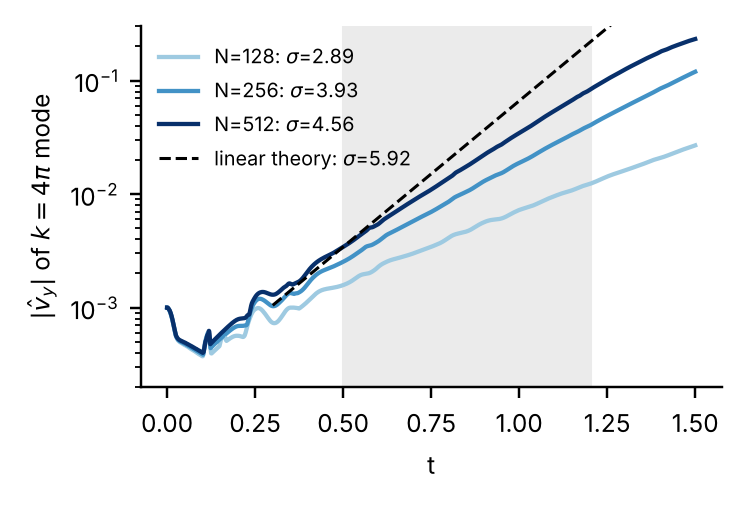
\includegraphics[width=\textwidth]{fig_growth.png}
\end{minipage}\hfill
\begin{minipage}{0.4\textwidth}
\small
\begin{tabular}{@{}lc@{}}
\toprule
Resolution & measured $\sigma$ \\
\midrule
$N=128$ & 2.89 \\
$N=256$ & 3.93 \\
$N=512$ & 4.56 \\
\midrule
extrapolated $N\to\infty$ & ${\approx}\,5.5$ \\
linear theory & 5.92 \\
\bottomrule
\end{tabular}
\end{minipage}
\caption{Growth of the seeded $k=4\pi$ mode ($w_0=10^{-3}$). Rates are fit over the shaded window, $0.5\le t\le1.2$. The extrapolation assumes $\sigma(N)=\sigma_\infty - C N^{-p}$, which gives $p\approx0.7$.}
\label{fig:growth}
\end{figure}

The measured rate \textbf{converges toward linear theory}: the gap to $5.92$ shrinks by about a third each time $N$ doubles, and the extrapolation lands within ${\sim}7\%$ of the theoretical value.

\section{5. Discussion}
\textbf{Why growth is slower than theory.} Numerical diffusion, mostly from the very dissipative Rusanov flux, smears the initially sharp interface over several cells. A shear layer of finite thickness $a$ is stabilized for $ka\gtrsim1$, so its growth falls below the vortex-sheet value. As $N$ grows the interface stays sharper and the rate climbs toward theory. Mild compressibility lowers it slightly further. The early dip at $t\lesssim0.4$ in Fig.~\ref{fig:growth} occurs because the seed is not an exact eigenmode of the problem.

\textbf{Why the fine structure doesn't converge.} The KH growth rate is proportional to $k$, so the smallest resolved scales always grow fastest. The instability therefore has no pointwise converged solution. Only statistical quantities, like the linear growth rate, converge, which is why it is the right quantity to test against.

\textbf{Limitations and next steps.} A fixed grid is not Galilean invariant: the error depends on how fast the gas moves relative to the grid. The Rusanov solver also smears contact discontinuities. Natural improvements are an HLLC Riemann solver, a smooth (tanh) initial shear layer for a cleaner comparison with linear theory, or a Galilean-invariant moving-mesh or meshless method (AREPO, GIZMO).


{\small\textbf{Code.} Adapted from \href{https://github.com/pmocz/finitevolume-python}{github.com/pmocz/finitevolume-python} (Mocz 2020). Figures and a movie: \texttt{KH\_finite\_volume.ipynb}.}
\end{document}
